\section{Transgressions and the Chern-Simons Form}
Notation: $\omega,\Omega$ are forms on the bundle $P$, while $A,F$ are forms on $M$.
\subsection{Gauss-Bonnet Theorem}
Our story begins with the Gauss-Bonnet theorem, which is a great theorem connecting 
local geometric quantity with global topologic quantity. 
\begin{theorem}[Gauss-Bonnet Theorem]
    Let $M^2$ be a closed oriented surface with Riemannian mertic, 
    $K$ be its Gauss curvature. Then 
    \begin{equation*}
        \frac{1}{2\pi}\int_M K \mathrm{dVol}_M = \chi(M),
    \end{equation*}
    where $\chi(M)$ is the Euler characteristic of $M$. If we denote the curvature 2-form of the Levi-Civita connection by $F$, 
    then $F = K \mathrm{dVol}_M$, thus we can rewrite the Gauss-Bonnet theorem as 
    \begin{equation*}
        \frac{1}{2\pi}\int_M F = \chi(M).
    \end{equation*}
\end{theorem}
To prove this theorem, we need to use the vector field $V$ on $M$.
\begin{definition}
    Let $V$ be a smooth vector field on $M$ with isolated zeros $\{x_i\}$. 
    % (We can start with a smooth vector field with isolated zeros and then normalize it.)
    On $M - \{x_i\}$, we can normalize $V$ to be a unit vector field $\tilde{V} = \frac{V}{|V|}$. 
    On each zero $x_i$, choose a small neighborhood $B_r(x_i)$, 
    then $\tilde{V}|_{\partial B_r(x_i)}$ can be viewed as a map from $S^1$ to $S^1$. 
    We define \emph{the index of $V$ at $x_i$} as the degree of this map, i.e.
    \begin{equation*}
        \mathrm{Ind}_{x_i}(V) = \deg(\tilde{V}|_{\partial B_r(x_i)}: S^1 \to S^1).
    \end{equation*}
    \emph{The index of $V$} is defined to be the sum of the indices at all zeros, 
    \begin{equation*}
        \mathrm{Ind}(V) = \sum_i \mathrm{Ind}_{x_i}(V).
    \end{equation*}
    The following picture shows some zeros with different indices.
    \begin{figure}[ht]
        \centering
        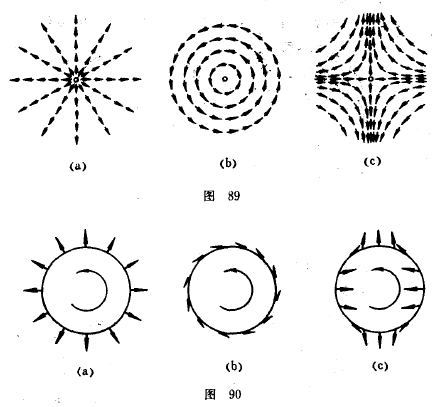
\includegraphics[scale=0.4]{Figures/Index-of-vector-field.png}
    \end{figure}
\end{definition}
\begin{remark}
    The index of $V$ at $x_i$ is independent of the choice of $B_r(x_i)$, thus is well-defined. 
    Since $\mathrm{Ind}(V)$ is an integer, it is invariant under homotopy of $V$. 
\end{remark}
\begin{theorem}(Poincar\'e-Hopf Index Theorem)
    Let $M$ be a closed oriented surface, $V$ be a smooth vector field on $M$ with isolated zeros. Then 
    \begin{equation*}
        \mathrm{Ind}(V) = \chi(M).
    \end{equation*}
\end{theorem}
\begin{proof}[Sketch of the proof]\hfill

    \textbf{Step 1: Independence of $V$.} Omit.
    % Let $V_1$ and $V_2$ be two normal vector fields on $M$ with isolated singular points. 
    % We can construct a polygonal decomposition of $M$ such that all singular points of $V_1$ and $V_2$ are contained in the interior of certain faces, 
    % and each faces contains at most one singular point. After a suitable homotopy, we can assume that $V_1$ and $V_2$ coincide on each vertex. 
    % \begin{figure}[h]
    %     \centering
    %     \includegraphics[scale=0.7]{Figures/PHthm1.png}
    %     \caption{Polygonal decomposition of $M$}
    % \end{figure}
    % Now for each edge $e$, pick an orientation of $e$, for example, from $v_1$ to $v_2$. 
    % We travel along $e$ from $v_1$ to $v_2$ and track $V_1$, then travel back from $v_2$ to $v_1$ and track $V_2$. 

    \textbf{Step 2: Construction of a special $V$.} Given a triangulation of $M$, we can construct a vector field $V$ such that 
    $\mathrm{Ind}(V) = \chi(M)$, thus we have $\mathrm{Ind}(V) = \chi(M)$ for any $V$. 
    The following picture shows how to construct such a vector field $V$: 
    \begin{figure}[ht]
        \centering
        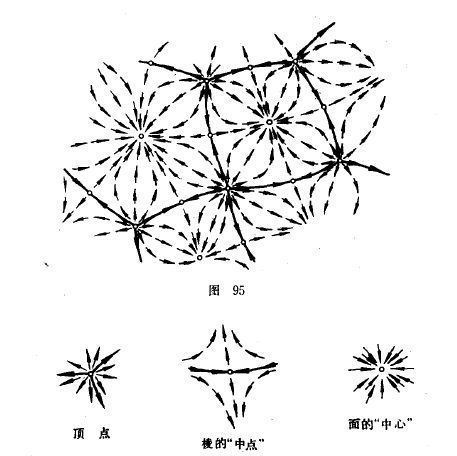
\includegraphics[scale=0.4]{Figures/PHthm2.png}
        % \caption{Polygonal decomposition of $M$}
    \end{figure}
\end{proof}

\begin{proof}[Proof of Gauss-Bonnet Theorem]
    Let $V$ be a smooth vector field on $M$ with isolated zeros $\{x_i\}$. 
    We construct another smooth vector field $W$ with the same zeros 
    such that $\{\tilde{V},\tilde{W}\}:=\{\frac{V}{|V|}, \frac{W}{|W|}\}$ is an orthonormal frame on $M - \{x_i\}$ compatible with the orientation of $M$. 

    Let $A$ be the connection 1-form of the Levi-Civita connection with respect to the frame $\{V,W\}$, i.e., 
    \begin{equation*}
        A(X):= \langle \nabla_X \tilde{V}, \tilde{W} \rangle, \quad \forall X \in T(M - \{x_i\}).
    \end{equation*}
    then the curvature 2-form $F = \mathrm{d}A$. Let $B_r(x_i)$ be a small neighborhood of $x_i$ containing no other zeros, then 
    \begin{align*}
        \frac{1}{2\pi}\int_M F &= \lim_{r\to 0} \frac{1}{2\pi}\int_{M - \cup_i B_r(x_i)} F \\ 
        &= \lim_{r\to 0} \frac{1}{2\pi}\int_{M - \cup_i B_r(x_i)} \mathrm{d}A \\ 
        &= \lim_{r\to 0} \sum_i \frac{1}{2\pi}\int_{\partial(M - B_r(x_i))} A \\ 
        &= \lim_{r\to 0} \sum_i \frac{1}{2\pi}\int_{\partial B_r(x_i)} A \\
    \end{align*}
    Notice that the left hand side is independent of the choice of metric and connection (by characteristic class theory), 
    thus we can choose any metric and connection we like. In particular, 
    we can choose the Euclidean metric and the trivial connection in each neighborhood $B_r(x_i)$. 
    Under a local coordinate system $(B_r(x_i); x, y)$, we can write 
    \begin{equation*}
        \tilde{V} = \cos\theta \pd{}{x} + \sin\theta \pd{}{y}, \quad \tilde{W} = -\sin\theta \pd{}{x} + \cos\theta \pd{}{y},
    \end{equation*}
    where $\theta = \theta(x,y)$ is a smooth function on $B_r(x_i)$. 
    Then 
    \begin{align*}
        A\left(\pd{}{x}\right) = \langle \nabla_{\pd{}{x}} \tilde{V}, \tilde{W} \rangle 
        = \langle -\theta_x\sin\theta \pd{}{x} + \theta_x\cos\theta \pd{}{y}, -\sin\theta \pd{}{x} + \cos\theta \pd{}{y} \rangle 
        = \theta_x, \\ 
        A\left(\pd{}{y}\right) = \langle \nabla_{\pd{}{y}} \tilde{V}, \tilde{W} \rangle 
        = \langle -\theta_y\sin\theta \pd{}{x} + \theta_y\cos\theta \pd{}{y}, -\sin\theta \pd{}{x} + \cos\theta \pd{}{y} \rangle 
        = \theta_y.
    \end{align*}
    Thus we have $A = \theta_x \mathrm{d}x + \theta_y \mathrm{d}y = \mathrm{d}\theta$, so 
    \begin{equation*}
        \lim_{r\to 0} \frac{1}{2\pi}\int_{\partial B_r(x_i)} A 
        = \lim_{r\to 0} \frac{1}{2\pi}\int_{\partial B_r(x_i)} \mathrm{d}\theta 
        = \mathrm{Ind}_{x_i}(V).
    \end{equation*}
    Therefore, 
    \begin{equation*}
        \frac{1}{2\pi}\int_M F = \sum_i \mathrm{Ind}_{x_i}(V) = \mathrm{Ind}(V) = \chi(M). \qedhere
    \end{equation*}
\end{proof}
\begin{remark}
    $A$ is not a globally defined 1-form on $M$, 
    but its exterior derivative $\md A$ can be extended to a globally defined 2-form on $M$.
\end{remark}
\subsubsection*{Gauss-Bonnet-Chern Theorem}
The Gauss-Bonnet-Chern theorem is a generalization of the Gauss-Bonnet theorem to higher dimensions. 
\begin{theorem}[Gauss-Bonnet-Chern Theorem]
    Let $M^{2n}$ be a closed oriented Riemannian manifold, 
    $F$ be the curvature 2-form of the Levi-Civita connection. Then 
    \begin{equation*}
        \int_M \mathrm{Pf}\left(\frac{F}{2\pi}\right) = \chi(M),
    \end{equation*}
    where $\mathrm{Pf}$ is the Pfaffian of a skew-symmetric matrix.
\end{theorem}
To prove this theorem, we need to use the following generalization of the Poincar\'e-Hopf index theorem. 
\begin{theorem}[General Poincar\'e-Hopf Index Theorem]
    Let $M$ be a closed oriented manifold, 
    $V$ be a smooth vector field on $M$ with isolated zeros. Then 
    \begin{equation*}
        \mathrm{Ind}(V) = \chi(M).
    \end{equation*}
\end{theorem}
\begin{proof}[Sketch of the proof]\hfill

    \textbf{Step 1: Independence of $V$.} Omit.

    \textbf{Step 2: Construction of a special $V$.} Choose $V$ to be the gradient vector field of a Morse function $f$ on $M$, 
    then the zeros of $V$ are exactly the critical points of $f$, 
    and the index of $V$ at a critical point $x_i$ is $(-1)^{\lambda_i}$, 
    where $\lambda_i$ is the Morse index of $x_i$. So 
    \begin{equation*}
        \mathrm{Ind}(V) = \sum_i (-1)^{\lambda_i} 
        = \sum_{\lambda}(-1)^{\lambda}\sharp\{\text{critical points of index }\lambda\} 
        = \chi(M). \qedhere
    \end{equation*}
\end{proof}
% We omit the proof of this theorem, and we sketch the proof of the Gauss-Bonnet-Chern theorem. 
\begin{proof}[Sketch of the proof of G.B.C. Theorem]
    Consider the unit sphere bundle $\pi_S: SM \to M$, 
    Chern constructed a global angular form $\Psi$ on $SM$ such that: 
    \begin{itemize}[leftmargin=*]
        \item $\Psi$ is the "transgression" of $\mathrm{Pf}\left(\frac{F}{2\pi}\right)$, i.e.,
        \begin{equation}\label{equ:transgression-in-GBC(1)}
            \mathrm{d}\Psi = \pi_S^* \mathrm{Pf}\left(\frac{F}{2\pi}\right). 
        \end{equation}
        \item For any $x \in M$, 
        \begin{equation}\label{equ:transgression-in-GBC(2)}
            \int_{S^{2n-1}_x} \iota_x^* \Psi = 1,
        \end{equation}
        where $\iota_x:S^{2n-1}_x \hookrightarrow SM$ is the inclusion of the fiber at $x$.
    \end{itemize}
    Now let $V$ be a normal vector field on $M$ with isolated singular points $\{x_i\}$. 
    $V$ can be viewed as a section of $SM$ over $M - \{x_i\}$. 
    Let $B_r(x_i)$ be a small neighborhood of $x_i$ containing no other singular points, then 
    \begin{align*}
        \int_M \mathrm{Pf}\left(\frac{F}{2\pi}\right) &= \lim_{r\to 0} \int_{M - \cup_i B_r(x_i)} \mathrm{Pf}\left(\frac{F}{2\pi}\right) \\ 
        &= \lim_{r\to 0} \int_{M - \cup_i B_r(x_i)} V^* \pi_S^* \mathrm{Pf}\left(\frac{F}{2\pi}\right) \\
        &= \lim_{r\to 0} \int_{M - \cup_i B_r(x_i)} V^* \mathrm{d}\Psi \\
        &= \lim_{r\to 0} \sum_i \int_{\partial(M - B_r(x_i))} V^* \Psi \\
        &= \lim_{r\to 0} \sum_i \int_{\partial B_r(x_i)} V^* \Psi \\
    \end{align*}
    Notice that the last integral actually computes the degree of $V|_{\partial B_r(x_i)}$, where
    \begin{equation*}
        V|_{\partial B_r(x_i)}: \partial B_r(x_i) \to SM|_{B_r(x_i)} \cong B_r(x_i) \times S^{2n-1} \simeq S^{2n-1},
    \end{equation*}
    Therefore, 
    \begin{equation*}
        \int_M \mathrm{Pf}\left(\frac{F}{2\pi}\right) = \sum_i \mathrm{deg}(V|_{\partial B_r(x_i)}) = \sum_i \mathrm{Ind}_{x_i}(V) = \mathrm{Ind}(V) = \chi(M). \qedhere
    \end{equation*}
\end{proof}
This proof highly depends on the magical construction of the global angular form $\Psi$, 
which is a special case of the transgression form we'll talk about later.
\begin{remark}
    Back in the 2-dimensional case, the unit sphere bundle $SM$ is just the oriented orthonormal frame bundle $SO(TM)$, 
    both of which are $S^1$-bundles over $M$. Let $\omega$ be the Ehresmann connection of $SO(TM)$ induced by the Levi-Civita connection, 
    $\Omega$ be the curvature of $\omega$. Since $SO(2)$ is abelian, we have 
    \begin{equation*}
        \Omega = \mathrm{d}\omega + \frac{1}{2}[\omega, \omega] = \mathrm{d}\omega, \qquad 
        \mathrm{Pf}\left(\frac{\Omega}{2\pi}\right) = \md\ \mathrm{Pf}\left(\frac{\omega}{2\pi}\right) =: \md\Psi.
    \end{equation*}
    The relation between $\Omega\in \Omega^2(SO(TM), \mathfrak{so}(2))$ and $F\in \Omega^2(M)$ is
    \begin{equation*}
        \mathrm{Pf}\left(\frac{\Omega}{2\pi}\right) = \pi_S^*\left(\frac{F}{2\pi}\right).
    \end{equation*}
    So 
    \begin{equation}\label{equ:transgression-in-2d(1)}
        \mathrm{d}\Psi = \pi_S^*\left(\frac{F}{2\pi}\right).
    \end{equation}
    Notice that the inclusion $\iota_x:S^1_x \hookrightarrow SO(TM)$ pulls back $\omega$ to 
    the Maurer-Cartan form $\omega_{MC}$ on $S^1$, where 
    \begin{align*}
        \omega_{MC} = g^{-1}\md g &= 
        \begin{pmatrix}
            \cos\theta & \sin\theta \\
            -\sin\theta & \cos\theta
        \end{pmatrix} \md 
        \begin{pmatrix}
            \cos\theta & -\sin\theta \\
            \sin\theta & \cos\theta
        \end{pmatrix} \\ 
        &= 
        \begin{pmatrix}
            \cos\theta & \sin\theta \\
            -\sin\theta & \cos\theta            
        \end{pmatrix}
        \begin{pmatrix}
            -\sin\theta\md\theta & -\cos\theta\md\theta \\
            \cos\theta\md\theta & -\sin\theta\md\theta
        \end{pmatrix} 
        = 
        \begin{pmatrix}
            0 & \md\theta \\
            -\md\theta & 0
        \end{pmatrix}
    \end{align*}
    Thus 
    \begin{equation}\label{equ:transgression-in-2d(2)}
        \iota_x^* \Psi = \iota_x^* \mathrm{Pf}\left(\frac{\omega}{2\pi}\right) = \mathrm{Pf}\left(\frac{\iota_x^* \omega}{2\pi}\right) 
        = \mathrm{Pf}\left(\frac{\omega_{MC}}{2\pi}\right) = \frac{\md\theta}{2\pi},
    \end{equation}
    is the angular form on $S^1_x$ with integral $1$. Formulars \eqref{equ:transgression-in-2d(1)} 
    and \eqref{equ:transgression-in-2d(2)} are exactly the properties of 
    the global angular form $\Psi$ in the proof of the G.B.C. theorem. 
    The form $A$ is just the pullback of $\Psi$ via the section $V:M-\{x_i\} \to SO(TM)$, i.e., $A = V^* \Psi$.
\end{remark}

\subsection{Transgressions} 
Now lets focus on a $G$-principal bundle $\pi: P \to M$ with connection $A$ and curvature $F$. 
The Chern-Weil theory tells us any invariant polynomial $\Phi$ on $\mathrm{Inv}^k(\mathfrak{g})$ defines
a closed $2k$-form $\Phi(F)$ on $M$ 
% \footnote{Although $\Phi(F)$ is actually defined on $P$, 
% we've shown that it is basic, thus can be pulled down as a form on $M$.} 
and its cohomology class $[\Phi(F)]$ is independent of the choice of connection. 

Consider the pullback bundle $\pi^*P$ over $P$, 
\begin{center}
    \begin{tikzcd}
    \pi^*P \arrow[d]   & P \arrow[d, "\pi"] \\
    P \arrow[r, "\pi"] & M                 
    \end{tikzcd}
\end{center}
$\pi^*P$ can be identified with the fiber product $P \times_M P$, 
thus has a tautological section $\Delta: P \to \pi^*P$, $\Delta(p) = (p,p)$. 
This means $\pi^*P$ is a trivial bundle, so all characteristic classes of $\pi^*P$ vanish. 
In particular, $[\Phi(\pi^*F)] = 0$ in $H^{2k}(P)$. 
Thus there exists a $(2k-1)$-form $\Psi(A,F)$ on $P$ such that
\begin{equation*}
    \mathrm{d}\Psi(A,F) = \Phi(\pi^*F) = \pi^* \Phi(F).
\end{equation*}
The form $\Psi(A,F)$ is called the \emph{transgression} of $\Phi(F)$. 

\begin{remark}
    Let $SO(TM)$ be the orthonormal frame bundle of a Riemannian manifold $M^{2n}$, 
    then the transgression of $\mathrm{Pf}\left(\frac{F}{2\pi}\right)\in \Omega^{2n}(M)$ is 
    a $(2n-1)$-form $\Psi$ on $SO(TM)$ such that $\mathrm{d}\Psi = \pi^* \mathrm{Pf}\left(\frac{F}{2\pi}\right)$.
    The unit sphere bundle $SM$ is the associated bundle of $SO(TM)$ with $SO(2n)$ naturally acting on $S^{2n-1}$, 
    thus we can induce a form $\tilde{\Psi}$ on $SM$ from $\Psi$. 
    It turns out that $\tilde{\Psi}$ is exactly the global angular form Chern constructed in the proof.
\end{remark}

There is a more explicit way to construct the transgression $\Psi(A,F)$. 
To introduce it, we need to review the Chern-Weil theory. 

Given two connection $\nabla_0$ and $\nabla_1$ on vector bundle $E$, 
the independence of characteristic classes on the choice of connection is proved by the following formula:
\begin{equation*}
    \Tr(\Omega_1^k) - \Tr(\Omega_0^k) 
    = \md\int_0^1 k\Tr\left(\dif{\omega_t}{t}\wedge\Omega_t^{k-1}\right) \md t. 
\end{equation*}
Here $\omega_t = (1-t)\omega_0 + t\omega_1$ is the connection form of $\nabla_t = (1-t)\nabla_0 + t\nabla_1$,
$\Omega_t$ is the curvature of $\nabla_t$. 
If we fix $\nabla_0$ to be flat, i,e., $\Omega_0 = 0$, 
then the right hand side exactly gives a transgression of $\Tr(\Omega_1^k)$.

\subsection{Chern-Simons Form}
Historically, Simons wanted to study the \emph{signature} of a 4-manifold $X^4$, 
which is related to the first Pontryagin class $p_1$ 
because of \textbf{the Hirzebruch signature theorem}:
\begin{equation*}
    \sigma(X) = \frac{1}{3}\int_X p_1(TX).
\end{equation*}
Notice that 
\begin{equation*}
    p_1(TX) = f_2\left(\frac{F}{2\pi}\right) 
    = \frac{1}{2}\left[\left(\Tr\left(\frac{F}{2\pi}\right)\right)^2
    -\Tr\left(\frac{F^2}{4\pi^2}\right)\right] 
    = -\frac{1}{8\pi^2}\Tr(F^2).
\end{equation*}
Simons constructed a transgression of $p_1(TX)$, which is now called the \emph{Chern-Simons form}. 

Let $M$ be a closed oriented 3-manifold, 
there is a fact that its oriented orthonormal frame bundle $SO(TM)$ is always trivial. 
So we can choose a global section $s: M \to SO(TM)$, 
and fix a trivial connection $\nabla_0$ on $SO(TM)$ such that 
its connection form is zero with respect to $s$. For any connection $\nabla_1$, 
let $A$ be its connection form with respect to $s$. 
Now the connection $\nabla_t = (1-t)\nabla_0 + t\nabla_1$ has connection form 
\begin{equation*}
    A_t = tA, 
\end{equation*}
and curvature
\begin{equation*}
    F_t = \md A_t + \frac{1}{2}[A_t, A_t] =
    t\mathrm{d}A + t^2 A \wedge A.
\end{equation*}
So the Chern-Simons form is
\begin{align}\label{equ:CS-form}
    -\frac{1}{8\pi^2}\int_0^1 k\Tr\left(\dif{A_t}{t}\wedge F_t^{k-1}\right) \md t 
    =& -\frac{1}{8\pi^2}\int_0^1 2\Tr\left(A \wedge\left(t\mathrm{d}A + t^2 A \wedge A\right)\right) \md t \tag*{} \\ 
    =& -\frac{1}{8\pi^2}\Tr\left(A \wedge \mathrm{d}A + \frac{2}{3}A \wedge A \wedge A\right).
\end{align}
\begin{remark}
    The Chern-Simons form is a 3-form on the oriented 3-manifold $M$. 
    It is closed for the dimension reason. 
\end{remark}
\begin{definition}[Chern-Simons functional]
    Let $M$ be a closed oriented 3-manifold, 
    $SO(TM)$ be its oriented orthonormal frame bundle, 
    $\nabla$ be a connection on $SO(TM)$. 
    For any global trivialization $s: M \to SO(TM)$,
    let $A$ be the connection form of $\nabla$ with respect to $s$, 
    then the \emph{Chern-Simons functional} of $\nabla$ is defined to be 
    \begin{equation*}
        CS(A) := \frac{1}{8\pi^2}\int_M \Tr\left(A \wedge \mathrm{d}A + \frac{2}{3}A \wedge A \wedge A\right).
    \end{equation*}
\end{definition}
\begin{remark}
    Notice that different choices of global trivialization $s,s'$ differ by a gauge transformation $g: M \to SO(3)$.
    One can show that although $CS(A)\neq CS(A')$ in general, but $CS(A) - CS(A')$ is always an integer. 
    Thus $CS(A)$ is well-defined as an element in $\mR/\mZ$. 
\end{remark}

\subsubsection*{Critical points of the Chern-Simons functional}
If the connection $\nabla$ is a critical point of the Chern-Simons functional.
Fix a global trivialization $s: M \to SO(TM)$ and let $A$ be the connection form of $\nabla$ w.r.t. $s$. 
Then for any variation $a \in \Omega^1(M, \mathfrak{so}(3))$, the perturbation $\nabla + ta$ has connection form $A + ta$, so
\begin{align*}
    &\left.\dif{}{t}\right|_{t=0}CS(A + ta) \\ 
    =& \dif{}{t}\Big|_{t=0} \frac{1}{8\pi^2}\int_M \Tr\left((A + ta) \wedge \mathrm{d}(A + ta) + \frac{2}{3}(A + ta) \wedge (A + ta) \wedge (A + ta)\right) \\ 
    =& \frac{1}{8\pi^2}\int_M \Tr\left(a \wedge \mathrm{d}A + A \wedge \mathrm{d}a + \frac{2}{3}(a \wedge A \wedge A + A \wedge a \wedge A + A \wedge A \wedge a)\right) \\ 
    =& \frac{1}{8\pi^2}\int_M \Tr\left(a \wedge \mathrm{d}A + \md(A\wedge a) + \md A\wedge a + 2a \wedge A \wedge A\right) \\ 
    =& \frac{1}{4\pi^2}\int_M \Tr\left(a \wedge (\md A + A\wedge A)\right) + \frac{1}{8\pi^2}\int_M \md\Tr\left(A\wedge a\right) \\ 
    =& \frac{1}{4\pi^2}\int_M \Tr\left(a \wedge F\right).
\end{align*}
Since $a$ is arbitrary, we have $F = 0$.
\begin{theorem}
    The critical points of the Chern-Simons functional are exactly the flat connections on $SO(TM)$.
\end{theorem}

\subsection{Gauge Transformation}
\begin{definition}
Let $\pi:P\to M$ be a $G$-principal bundle, the \emph{gauge transformation} of $P$ is a $G$-bundle automorphism $\varphi: P \to P$, 
i.e., $\varphi$ is a diffeomorphism such that $\varphi(pg) = \varphi(p)g$ and $\pi \circ \varphi = \pi$. 
\begin{center}
    \begin{tikzcd}
    P \arrow[rd, "\pi"'] \arrow[rr, "\varphi"] &   & P \arrow[ld, "\pi"] \\
                                            & M &                    
    \end{tikzcd}
\end{center}
All gauge transformations of $P$ form the \emph{gauge group} of $P$, denoted by $\mathcal{G}(P)$.
\end{definition}
\begin{example}
    For trivial bundle $P = M \times G$, each smooth function $f: M \to G$ defines a gauge transformation $\varphi(x,g) = (x, f(x)g)$. 
    In fact, all gauge transformations are of this form, so $\mathcal{G}(M\times G) \cong C^{\infty}(M,G)$, 
    where multiplication in $C^{\infty}(M,G)$ is defined pointwise.
\end{example}

Let $\varphi: P \to P$ be a gauge transformation, 
then for any $p\in P$, there exists a unique $g_p \in G$ such that $\varphi(p) = p g_p$. 
Thus we can define a smooth function $f: P \to G$ by $f(p) = g_p$.
\begin{proposition}
    $f:P\to G$ defined above satisfies $f(pg) = g^{-1}f(p)g,\,\forall\,p\in P,g\in G$.
\end{proposition}
\begin{proof}
    Since $\varphi$ is $G$-equivariant, 
    \begin{equation*}
        pgf(pg) = \varphi(pg) = \varphi(p)g = pf(p)g
        \implies f(pg) = g^{-1}f(p)g. \qedhere
    \end{equation*}
\end{proof}
The above proposition implies that $f$ can be viewed as a section of 
the associated bundle $\mathrm{Ad}P := P \times_{\mathrm{cong}} G$ 
with $G$ acting on itself by conjugation. 
\begin{theorem}
    There is a one-to-one correspondence between the gauge group $\mathcal{G}(P)$ and the space of sections $C^{\infty}(M, \mathrm{Ad}P)$. 
    If we define the multiplication in $C^{\infty}(M, \mathrm{Ad}P)$ pointwise, then this correspondence is a group isomorphism.
\end{theorem}
\begin{proof}
    \begin{equation*}
        \left\{
            \begin{array}{c}
                \text{sections of } \mathrm{Ad}P \\[2pt]
                s: M \to \mathrm{Ad}P
            \end{array}
        \right\} \overset{\text{1-1}}{\longleftrightarrow}
        \left\{
            \begin{array}{c}
                \text{G-equivariant maps} \\[2pt]
                f: P \to G
            \end{array}
        \right\} \overset{\text{1-1}}{\longleftrightarrow}
        \left\{
            \begin{array}{c}
                \text{gauge transformations} \\[2pt]
                \varphi(p) = p f(p)
            \end{array}
        \right\}.
    \end{equation*}
\end{proof}
\begin{example}
    For the trivial bundle $P = M \times G$, we have $\mathrm{Ad}P = M \times G$, 
    so $C^{\infty}(M, \mathrm{Ad}P) \cong C^{\infty}(M,G)$. 
\end{example}
\begin{example}
    For abelian $G$, the conjugation action is trivial, 
    so $\mathrm{Ad}P = P \times_{\mathrm{cong}} G \cong M \times G$, 
    thus $\mathcal{G}(P) \cong C^{\infty}(M,G)$.
\end{example}
\subsubsection*{Gauge transformation acts on connections}
Let $\varphi: P \to P$ be a gauge transformation,
then for any connection $\omega$ on $P$, 
we can pull back $\omega$ via $\varphi$ to get $\varphi^* \omega$. 
\begin{theorem}
    $\varphi^* \omega$ is still a connection on $P$.
\end{theorem}
\dots
\subsection{Holonomy and flat connections}
\dots